%!TeX root=../tese.tex

\chapter{Appendices}

\section{Proofs}

\begin{theorem}
  \label{thm:summix}
  Let $\mathcal{C}$ a probabilistic circuit whose first $l$ layers are composed solely of sum
  nodes. Call $\Nodes$ the set of all nodes in layer $l+1$. $\mathcal{C}$ is equivalent to a PC
  $\mathcal{C}'$ whose root is a sum node with $\Nodes$ as children.
\end{theorem}
\begin{proof}
  We adapt a similar proof due to \citet{jaini18b}. Every sum node is of the form
  \begin{equation*}
    \Sum(\set{x})=\sum_{\Child\in\Ch(\Sum)}w_{\Sum,\Child}\cdot\Child(\set{x}).
  \end{equation*}
  Particularly, every child $\Child$ in a sum node in layer $1\leq i\leq l-1$, is a sum node, and
  so for the first layer we have that
  \begin{align*}
    \Sum(\set{x})&=\sum_{\Child_1\in\Ch(\Sum)}w_{\Sum,\Child_1}\sum_{\Child_2\in\Ch(\Child_1)}
    w_{\Child_1,\Child_2}\Child_2(\set{x})\\
                 &=\sum_{\Child_1\in\Ch(\Sum)}\sum_{\Child_2\in\Ch(\Child_1)}w_{\Sum,\Child_1}
    w_{\Child_1,\Child_2}\Child_2(\set{x}).
  \end{align*}
  Define a one-to-one mapping that takes a tuple $(\Child_1,\Child_2)$ where $\Child_1\in\Ch(\Sum)$
  and $\Child_2\in\Ch(\Child_1)$ and returns a (unique) path from $\Sum$ to every grandchild
  $\Child_2$ of $\Sum$. Call $\set{K}$ the set of all paths, and $w_{\Sum,\Child_1}$ and
    $w_{\Child_1,\Child_2}$ the weights for one such path. We can merge these two weights into a
  single weight $w_{\Sum,\Child_2}'= w_{\Sum,\Child_1}\cdot w_{\Child_1,\Child_2}$, yielding
  \begin{equation*}
    \Sum(\set{x})=\sum_{(w_{\Sum,\Child_1},w_{\Child_1,\Child_2})\in\set{K}} w_{\Sum,\Child_2}'
    \Child_2(\set{x}).
  \end{equation*}
  This ensures that two consecutive sum layers can be collapsed into a single layer. Particularly,
  for the first (root) and second layers, the above transformation generates a circuit with one
  fewer layer and whose root has $\bigo(nm)$ edges, where $n$ and $m$ are the number of edges coming
  from the original root and its children respectively. We can apply this procedure until there are
  no more consecutive sum nodes. This results in a PC of the form
  \begin{equation*}
    \Sum(\set{x})=\sum_{\Child\in\Ch(S)} w_{\Sum,\Child}\Node(\set{x}),
  \end{equation*}
  where $\Node\in\Nodes$. The number of children of the resulting root sum node will be exponential
  on the number of edges of its children.
\end{proof}

\begin{theorem}[Standardization]
  \label{thm:standard}
  Any probabilistic circuit $\mathcal{C}$ can be reduced to a circuit where every sum node contains
  only products or inputs and every product node contains only sums or inputs.
\end{theorem}
\begin{proof}
  If $\mathcal{C}$ is already standard we are done. Otherwise, there exists either (i) a sum node
  $\Sum$ with a sum $\Sum'$ as child; or (ii) a product node $\Prod$ with a product $\Prod'$ as
  child. We first address (i): let $w$ be the weight of edge $\edge{\Sum\Sum'}$ and $\theta_i$
  the weights from all edges coming out from $\Sum'$.
  \begin{center}
    \begin{tikzpicture}
      \newSumNode[label=above right:{$\Sum$}]{s}{0,0};
      \newProdNode{p1}{$(s) + (-1.25,-1)$};
      \newSumNode[label=above left:{$\Sum'$}]{sl}{$(s) + (0,-1.5)$};
      \newProdNode{p2}{$(s) + (1.25,-1)$};
      \newProdNode{q1}{$(sl) + (-1.25,-1)$};
      \newProdNode{q2}{$(sl) + (0,-1)$};
      \newProdNode{q3}{$(sl) + (1.25,-1)$};
      \draw[edge] (s) edge (p1);
      \draw[edge] (s) edge node[midway,right] {\scriptsize$w$} (sl);
      \draw[edge] (s) edge (p2);
      \draw[edge] (sl) edge node[midway,left] {\scriptsize$\theta_1$} (q1);
      \draw[edge] (sl) edge node[midway,left] {\scriptsize$\theta_2$} (q2);
      \draw[edge] (sl) edge node[midway,left] {\scriptsize$\theta_3$} (q3);

      \draw[edge,very thick,red] (2.25,-1.5) -- node[midway,above] {Standardize} (5.5,-1.5);

      \newSumNode[label=above right:{$\Sum$}]{s}{8,0};
      \newProdNode{p1}{$(s) + (-1.5,-1.0)$};
      \newProdNode{p2}{$(s) + (1.5,-1.0)$};
      \newProdNode{q1}{$(s) + (-1.5,-2.5)$};
      \newProdNode{q2}{$(s) + (-0,-2.5)$};
      \newProdNode{q3}{$(s) + (1.5,-2.5)$};
      \draw[edge] (s) edge (p1);
      \draw[edge] (s.south) -- ++(0,-1.25) -| node[midway,below right] {\scriptsize$w\cdot\theta_1$} (q1);
      \draw[edge] (s.south) -- ++(0,-1.25) -| node[midway,below right] {\scriptsize$w\cdot\theta_2$} (q2);
      \draw[edge] (s.south) -- ++(0,-1.25) -| node[midway,below right] {\scriptsize$w\cdot\theta_3$} (q3);
      \draw[edge] (s) edge (p2);
    \end{tikzpicture}
  \end{center}
  Connect $\Sum$ with every child of $\Sum'$, assigning as weight $w\cdot\theta_i$ for each child
  $i$. Delete $\Sum'$ and all edges coming out from it. The resulting circuit is computationally
  equivalent but now without a consecutive pair of sums. This transformation is visualized by the
  figure above. We do a similar procedure in (ii), but now instead remove $\Prod'$ and connect all
  children of $\Prod'$ to $\Prod$, as we show below.
  \begin{center}
    \begin{tikzpicture}
      \newProdNode[label=above right:{$\Prod$}]{s}{0,0};
      \newSumNode{p1}{$(s) + (-1.25,-1)$};
      \newProdNode[label=above left:{$\Prod'$}]{sl}{$(s) + (0,-1.5)$};
      \newSumNode{p2}{$(s) + (1.25,-1)$};
      \newSumNode{q1}{$(sl) + (-1.25,-1)$};
      \newSumNode{q2}{$(sl) + (0,-1)$};
      \newSumNode{q3}{$(sl) + (1.25,-1)$};
      \draw[edge] (s) edge (p1);
      \draw[edge] (s) edge (sl);
      \draw[edge] (s) edge (p2);
      \draw[edge] (sl) edge (q1);
      \draw[edge] (sl) edge (q2);
      \draw[edge] (sl) edge (q3);

      \draw[edge,very thick,red] (2.25,-1.5) -- node[midway,above] {Standardize} (5.5,-1.5);

      \newProdNode[label=above right:{$\Prod$}]{s}{8,0};
      \newSumNode{p1}{$(s) + (-1.5,-1.0)$};
      \newSumNode{p2}{$(s) + (1.5,-1.0)$};
      \newSumNode{q1}{$(s) + (-1.5,-2.5)$};
      \newSumNode{q2}{$(s) + (-0,-2.5)$};
      \newSumNode{q3}{$(s) + (1.5,-2.5)$};
      \draw[edge] (s) edge (p1);
      \draw[edge] (s.south) -- ++(0,-1.25) -| (q1);
      \draw[edge] (s.south) -- ++(0,-1.25) -| (q2);
      \draw[edge] (s.south) -- ++(0,-1.25) -| (q3);
      \draw[edge] (s) edge (p2);
    \end{tikzpicture}
  \end{center}
\end{proof}

\begin{theorem}[2-Standardization]
\label{thm:2standard}
Any probabilistic circuit $\mathcal{C}$ can be transformed into a circuit where every sum node
contains only products or inputs and every product node contains only \emph{two} sums or inputs.
\end{theorem}
\begin{proof}
  For sums, apply the same standardization procedure as \Cref{thm:standard}. Let $\Prod$ a product
  and call $n=|\Ch(\Prod)|$. If $n=1$ and $\Ch(\Prod)$ is a product, then remove $\Prod$ and
  connect all previous parents of $\Prod$ with its child. If $n=1$ and $\Ch(\Prod)$ is not a
  product, remove $\Prod$ and apply the standardization procedure for sums on all of $\Pa(\Prod)$.

  For $n>2$, we simply need to split into 2-products recursively. We prove this by induction. The
  base case is when $n=2$, which is already done, or $n=3$, in which case we need apply the
  transformation below.
  \begin{center}
    \begin{tikzpicture}
      \newProdNode{r}{0,0};
      \newSumNode{s1}{$(r) + (-1.5,-2)$};
      \newSumNode{s2}{$(r) + (0,-2)$};
      \newSumNode{s3}{$(r) + (1.5,-2)$};
      \draw[edge] (r) -- (s1);
      \draw[edge] (r) -- (s2);
      \draw[edge] (r) -- (s3);

      \draw[edge,very thick,red] (2.25,-0.5) -- node[midway,above] {2-Standardize} (5.5,-0.5);

      \newProdNode{r}{7,0};
      \newSumNode[fill=boxorange!80]{t}{$(r) + (-0.5,-1)$};
      \newSumNode{s1}{$(r) + (0.5,-1)$};
      \newProdNode[fill=boxgoldenrod!70]{p}{$(t) + (-0.5,-1)$};
      \newSumNode{s2}{$(p) + (-0.5,-1)$};
      \newSumNode{s3}{$(p) + (0.5,-1)$};
      \draw[edge] (r) -- (t);
      \draw[edge] (r) -- (s1);
      \draw[edge] (t) -- (p);
      \draw[edge] (p) -- (s2);
      \draw[edge] (p) -- (s3);
    \end{tikzpicture}
  \end{center}
  Where \inode[fill=boxorange!80]{\newSumNode} and \inode[fill=boxgoldenrod!70]{\newProdNode} are
  newly introduced nodes. When $n>3$, we create two products $\Prod_1$ and $\Prod_2$, each
  connected with a sum and product, and with $\left\lfloor\frac{n}{2}\right\rfloor$ and
  $\left\lceil\frac{n}{2}\right\rceil$ potential children. By the induction hypothesis, we can
  recursively binarize the subsequent grandchildren products.
  \begin{center}
    \begin{tikzpicture}
      \newProdNode{r}{0,0};
      \newSumNode{s1}{$(r) + (-2,-2)$};
      \newSumNode{s2}{$(r) + (-1,-2)$};
      \newSumNode{s3}{$(r) + (0,-2)$};
      \newSumNode{s4}{$(r) + (1,-2)$};
      \newSumNode{s5}{$(r) + (2,-2)$};
      \draw[edge] (r) -- (s1);
      \draw[edge] (r) -- (s2);
      \draw[edge] (r) -- (s3);
      \draw[edge] (r) -- (s4);
      \draw[edge] (r) -- (s5);

      \draw[edge,very thick,red] (2.25,-0.5) -- node[midway,above] {2-Standardize} (5.5,-0.5);

      \newProdNode{r}{7,0};
      \newSumNode[fill=boxorange!80]{t1}{$(r) + (-0.5,-1)$};
      \newSumNode[fill=boxorange!80]{t2}{$(r) + (0.5,-1)$};
      \newProdNode[fill=boxgoldenrod!70]{p1}{$(t1) + (-0.5,-1)$};
      \newProdNode[fill=boxgoldenrod!70]{p2}{$(t2) + (0.5,-1)$};
      \newSumNode{s1}{$(p1) + (-0.5,-1)$};
      \newSumNode{s2}{$(p1) + (0.5,-1)$};
      \newSumNode{s3}{$(p2) + (-0.75,-1)$};
      \newSumNode{s4}{$(p2) + (0.0,-1)$};
      \newSumNode{s5}{$(p2) + (0.75,-1)$};
      \draw[edge] (r) -- (t1);
      \draw[edge] (r) -- (t2);
      \draw[edge] (t1) -- (p1);
      \draw[edge] (t2) -- (p2);
      \draw[edge] (p1) -- (s1);
      \draw[edge] (p1) -- (s2);
      \draw[edge] (p2) -- (s3);
      \draw[edge] (p2) -- (s4);
      \draw[edge] (p2) -- (s5);
    \end{tikzpicture}
  \end{center}
  As an example, we have $n=5$ in the figure above. We introduce the sums
  \inode[fill=boxorange!80]{\newSumNode} and products \inode[fill=boxgoldenrod!70]{\newProdNode}
  and then recursively apply the transformation again on the
  \inode[fill=boxgoldenrod!70]{\newProdNode}s.

  When $\Ch(\Prod)$ are product nodes we do the same procedure as before, but with the added
  post-process addition of a sum node connecting \inode[fill=boxgoldenrod!70]{\newProdNode} to
  every $\Ch(\Prod)$.
\end{proof}

\linevi*
\begin{proof}
  \label{proof:linevi}
  For a sum node $\Sum$ and query variables $\set{X}$, we have the following marginalization of
  variables $\set{Y}$
  \begin{align*}
    \int\Sum(\set{x},\set{y})\dif\set{y}&=\int\sum_{\Child\in\Ch(\Sum)}w_{\Sum,\Child}\Child(\set{x},\set{y})\dif\set{y}\\
                                        &=\sum_{\Child\in\Ch(\Sum)}w_{\Sum,\Child}\int\Child(\set{x},\set{y})\dif\set{y}.
  \end{align*}
  Analogously, for a product node
  \begin{align*}
    \int\Prod(\set{x},\set{y})\dif\set{y}&=\int\prod_{\Child\in\Ch(\Prod)}\Child(\set{x},\set{y})\dif\set{y}\\
                                         &=\prod_{\Child\in\Ch(\Prod)}\int\Child(\set{x},\set{y})\dif\set{y}.
  \end{align*}
  This ensures that marginals are pushed down to children. This can be done recursively until
  $\Child$ is an input node $\Leaf_p$, in which case we marginalize $\set{y}$ according to $p$,
  which by definition should be tractable and here we assume can be done in $\bigo(1)$. We have
  proved the case for \mar{}. For \evi{}, we simply assign $\set{y}=\emptyset$ with input nodes
  acting as probability density functions. Conditionals can easily be computed by an \evi{} or
  \mar{} followed by a second pass marginalizing the conditional variables
  $p(\set{x}|\set{y})=\frac{p(\set{x},\set{y})}{p(\set{y})}$ which are both done in linear time as
  we have seen here.
\end{proof}

\det*
\begin{proof}
  \label{proof:det}
  For a sum node $\Sum$, we want to compute the following query
  \begin{equation*}
    \max_{\set{y}}\Sum(\set{y}|\set{x})=\frac{1}{\Sum(\set{x})}\max_{\set{y}}\Sum(\set{y},\set{x})
    =\frac{1}{\Sum(\set{x})}\max_{\set{y}}\sum_{\Child\in\Ch(\Sum)}w_{\Sum,\Child}\Child(\set{y},\set{x}),
  \end{equation*}
  yet notice that for any assignment of $\set{x}$ and $\set{y}$ only one $\Child\in\Ch(\Sum)$ must
  have a nonnegative value by the definition of determinism, so we may replace the summation with
  a maximization over the children, giving
  \begin{equation*}
    \max_{\set{y}}\Sum(\set{y}|\set{x})=\frac{1}{\Sum(\set{x})}\max_{\set{y}}\max_{\Child\in\Ch(\Sum)}w_{\Sum,\Child}\Child(\set{y},\set{x})
    =\frac{1}{\Sum(\set{x})}\max_{\Child\in\Ch(\Sum)}\max_{\set{y}}w_{\Sum,\Child}\Child(\set{y},\set{x}).
  \end{equation*}
  For a product node $\Prod$, we compute
  \begin{align*}
    \max_{\set{y}}\Prod(\set{y}|\set{x})=\frac{1}{\Prod(\set{x})}\max_{\set{y}}\Prod(\set{y},\set{x})
    =\frac{1}{\Prod(\set{x})}\max_{\set{y}}\prod_{\Child\in\Ch(\Prod)}\Child(\set{y},\set{x})
    =\frac{1}{\Prod(\set{x})}\prod_{\Child\in\Ch(\Prod)}\max_{\set{y}}\Child(\set{y},\set{x}).
  \end{align*}
  This is equivalent to an inductive top-down pass where we maximize instead of sum until we reach
  all input nodes, in which case we simply maximize the supposedly tractable functions. Once these
  are computed, we unroll the induction, maximizing over all values.
\end{proof}

\expcthm*
\begin{proof}
  For completeness, we show the proof of this claim as stated in \cite{choi20}. We assume, without
  loss of generality, that the layers of both $\mathcal{C}$ and $\mathcal{L}$ are compatible, i.e.\
  they both have the same number of layers and if the $i$-th layer of $\mathcal{C}$ is made out of
  sums (resp. products), then the $i$-th layer of $\mathcal{L}$ is made out of disjunctions (resp.
  conjunctions). The expectation $\mathbb{E}_\mathcal{C}\left[\mathcal{L}\right]$ has the following
  form when the root of $\mathcal{C}$ is a product
  \begin{align*}
    \mathbb{E}_\mathcal{C}\left[\mathcal{L}\right]&=\int\mathcal{C}(\set{x})\mathcal{L}(\set{x})\dif\set{x}=
    \int\left(\mathcal{C}_p(\set{x})\mathcal{C}_s(\set{x})\right)
    \left(\mathcal{L}_p(\set{x})\mathcal{L}_s(\set{x})\right)\dif\set{x}\\
    &=\int\left(\mathcal{C}_p(\set{x})\mathcal{L}_p(\set{x})\right)\left(\mathcal{C}_s(\set{x})\mathcal{L}_s(\set{x})\right)\dif\set{x}
    =\int\left(\mathcal{C}_p(\set{x})\mathcal{L}_p(\set{x})\right)\dif\set{x}
    \int\left(\mathcal{C}_s(\set{x})\mathcal{L}_s(\set{x})\right)\dif\set{x}\\
    &=\mathbb{E}_{\mathcal{C}_p}\left[\mathcal{L}_p\right]\cdot\mathbb{E}_{\mathcal{C}_s}\left[\mathcal{L}_s\right],
  \end{align*}
  where the subscript $p$ and $s$ indicate the prime and sub of a node. When the root is a sum
  \begin{align*}
    \mathbb{E}_\mathcal{C}\left[\mathcal{L}\right]&=\int\mathcal{C}(\set{x})\mathcal{L}(\set{x})\dif\set{x}
    =\int\left(\sum_{\Child'\in\Ch(\mathcal{C})}w_{\mathcal{C},\Child'}\Child'(\set{x})\right)
    \left(\sum_{\Child''\in\Ch(\mathcal{L})}\Child''(\set{x})\right)\dif\set{x}\\
    &=\int\sum_{\Child'\in\Ch(\mathcal{C})}\sum_{\Child''\in\Ch(\mathcal{L})}w_{\mathcal{C},\Child'}\cdot\Child'(\set{x})\cdot\Child''(\set{x})\dif\set{x}
    =\sum_{\Child'\in\Ch(\mathcal{C})}\sum_{\Child''\in\Ch(\mathcal{L})}w_{\mathcal{C},\Child'}\int\Child'(\set{x})\Child''(\set{x})\dif\set{x}\\
    &=\sum_{\Child'\in\Ch(\mathcal{C})}\sum_{\Child''\in\Ch(\mathcal{L})}w_{\mathcal{C},\Child'}\cdot\mathbb{E}_{\Child'}\left[\Child''\right].
  \end{align*}
  Therefore, if expectation is tractable for input nodes, then expectation is tractable for the
  whole circuit.
\end{proof}

\section{\textproc{SamplePSDD}}
\label{sec:samplepsdd-app}

We now transcribe the supplemental material found in \citet{geh21a}. In this section, we describe a
fast implementation of \textproc{SamplePSDD} that avoids the use of the costly Forget operation. We
then show additional experiments with \num{1000} iterations of \textproc{LearnPSDD} and
\textproc{Strudel}, followed by the complete log-likelihood results in table form. Finally, we list
in more detail the logical constraints used in each of the domains described in
\Cref{sec:logical-exp}.

\subsection{Fast implementation of \textsc{SamplePSDD}}

In order to produce valid (partial) partitions, \textsc{SamplePSDD} requires that the
\textsc{Forget} operation be called for every sub lest the scope of the formula contradicts the
respective scope in vtree. Despite \textsc{Forget} taking polynomial time in the size of the BDD,
we can make sampling more efficient by directly ``forgetting''  a variable when returning a PSDD
structure. \Cref{alg:fastsamplepsdd} modifies \Cref{alg:samplepsdd} to handle variables not
appearing in the formula $\phi$. Lines 2 -- 7 ensure that the formula correctly accounts for the
forgetting of variables not in the scope of the vtree. Hence, we can omit the \textsc{Forget}
operation in \Cref{alg:samplepartial}, resulting in \Cref{alg:samplepartial-fast}. Since the
restricion $\psi|X$ is linearithmic in the size of the BDD, and constructing a conjunction of
literals $\alpha$ is linear in $|\Sc(\alpha)|$, the algorithm is highly efficient.

\setcounter{algorithm}{20}
\begin{algorithm}
  \caption{\textproc{FastSamplePSDD}}\label{alg:fastsamplepsdd}
  \begin{algorithmic}[1]
    \Require BDD $\phi$, vtree node $v$, number of primes $k$
    \Ensure A sampled PSDD structure
    \If{$v$ is a leaf}
      \If{$v\in\phi$}
        \IIf{$\phi$ is a literal}{\textbf{return} $\phi$ as a literal node}
        \IIf{$\phi|_v\equiv\top$}{\textbf{return} $v$ as a literal node}
        \IIf{$\phi|_{\neg v}\equiv\top$}{\textbf{return} $\neg v$ as a literal node}
      %\Else \textbf{ return} a Bernoulli over $v$ 
      \EndIf
        \State \textbf{return} a Bernoulli over $v$
    \ElsIf{$\phi\equiv\top$}
      \State \textbf{return} a fully factorized circuit over $\Sc(v)$
    \EndIf
    \State $\set{E}\gets\Call{FastSamplePartialPartition}{\phi,\Sc(v^{\gets}),k}$
    \State Create an OR gate $\Sum$
    \State Randomly compress elements in $\set{E}$ with equal subs
    \State Randomly merge elements in $\set{E}$ with equal subs
    \For{each element $(p,s)\in\set{E}$}
      \State $l\gets\Call{SampleExactPSDD}{p,v^\gets,k}$
      \State $r\gets\Call{FastSamplePSDD}{s,v^\to,k}$
      \State Add an AND gate with inputs $l$ and $r$ as a child of $\Sum$
    \EndFor
    \State \textbf{return} $\Sum$
  \end{algorithmic}
\end{algorithm}

\begin{algorithm}[t]
  \caption{\textproc{FastSamplePartialPartition}}\label{alg:samplepartial-fast}
  \begin{algorithmic}[1]
    \Require BDD $\phi$, vtree node $v$, number of primes $k$
    \Ensure A set of sampled elements
    \State Define $\set{E}$ as an empty collection of sampled elements
    \State Sample an ordering $X_1,\dotsc,X_m$ of $\Sc(v^\gets)\cap\Sc(\phi)$
    \State Let $\set{Q}$ be a queue initially containing $(\phi,1,\{\})$
    \State $j\gets 1$ \Comment{Counter of sampled elements}
    \While{$|\set{E}|<k$}
      \State Pop top item $(\psi,i,p)$ from $\set{Q}$
      \If{$j\geq k$ or $i>m$ or $\psi\equiv\top$}
%        \State Define $e\gets\left(\bigwedge_{X\in\set{V}}X,\Forget(\phi|_{\set{V}},\Sc(v^\gets))\right)$
 %       \State Add new element $e$ to $\set{E}$
        \State Add $\left(p,\phi|_{p}\right)$ to $\set{E}$
        \State \textbf{continue}
      \EndIf
      %\State Let $X$ be the $i$-th variable in $\set{O}$
      \State $\alpha\gets\psi|_{X_i}$, $\beta\gets\psi|_{\neg X_i}$
      \If{$\alpha \equiv \beta$} enqueue $(\psi,i+1,p)$ in $\set{Q}$
      \Else
        \IIf{$\alpha\not\equiv\bot$}{push $(\alpha,i+1,p \wedge X_i)$ to $\set{Q}$}
        \IIf{$\beta\not\equiv\bot$}{push $(\beta,i+1,p\wedge\neg X_i)$ to $\set{Q}$}
        \State $j\gets j+1$
      \EndIf
    \EndWhile
    \State \textbf{return} $\set{E}$
  \end{algorithmic}
\end{algorithm}

\subsection{Additional Experiments}

We repeat the accuracy vs.\  sample size plots including the results of running \textsc{Strudel}
and \textsc{MixStrudel} for 1000 iterations, as used in the original paper. \Cref{fig:performance}
shows all results with the added Strudel and MixStrudel with 1000 iterations curves.

\begin{figure*}
  \begin{subfigure}[b]{0.495\textwidth}
    \centering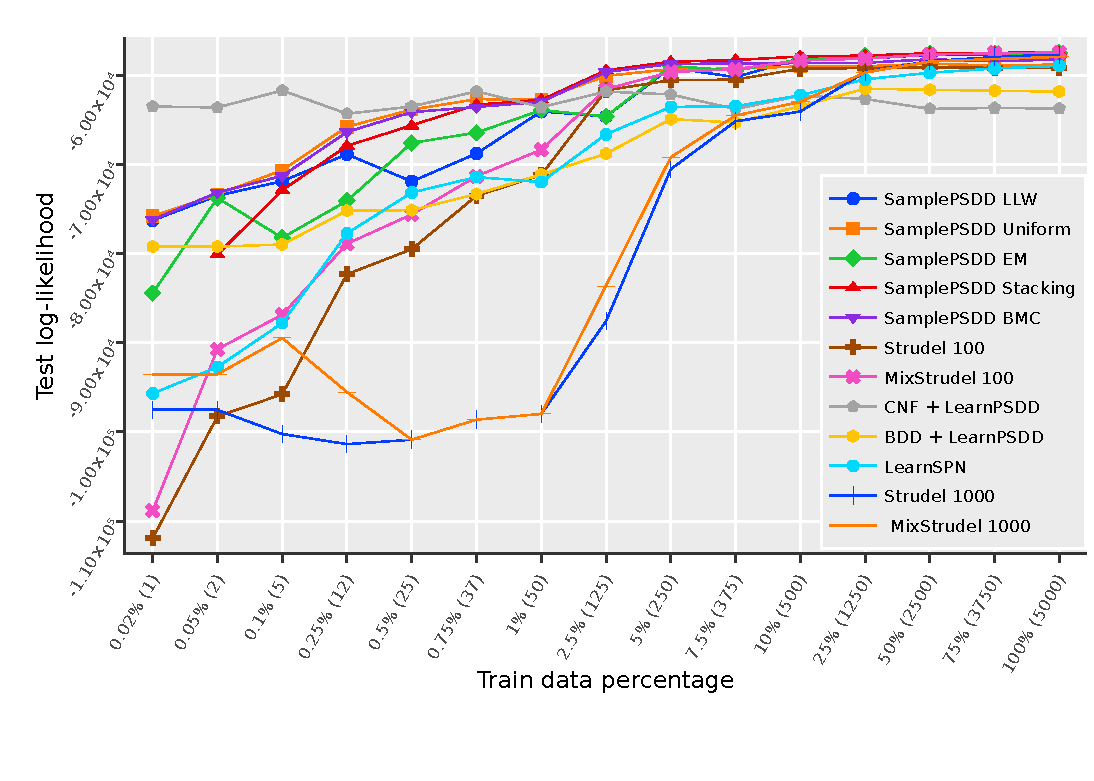
\includegraphics[width=\textwidth]{supplementary/all_ll_led_ensembles.pdf}
    \caption{}
  \end{subfigure}
  \begin{subfigure}[b]{0.495\textwidth}
    \centering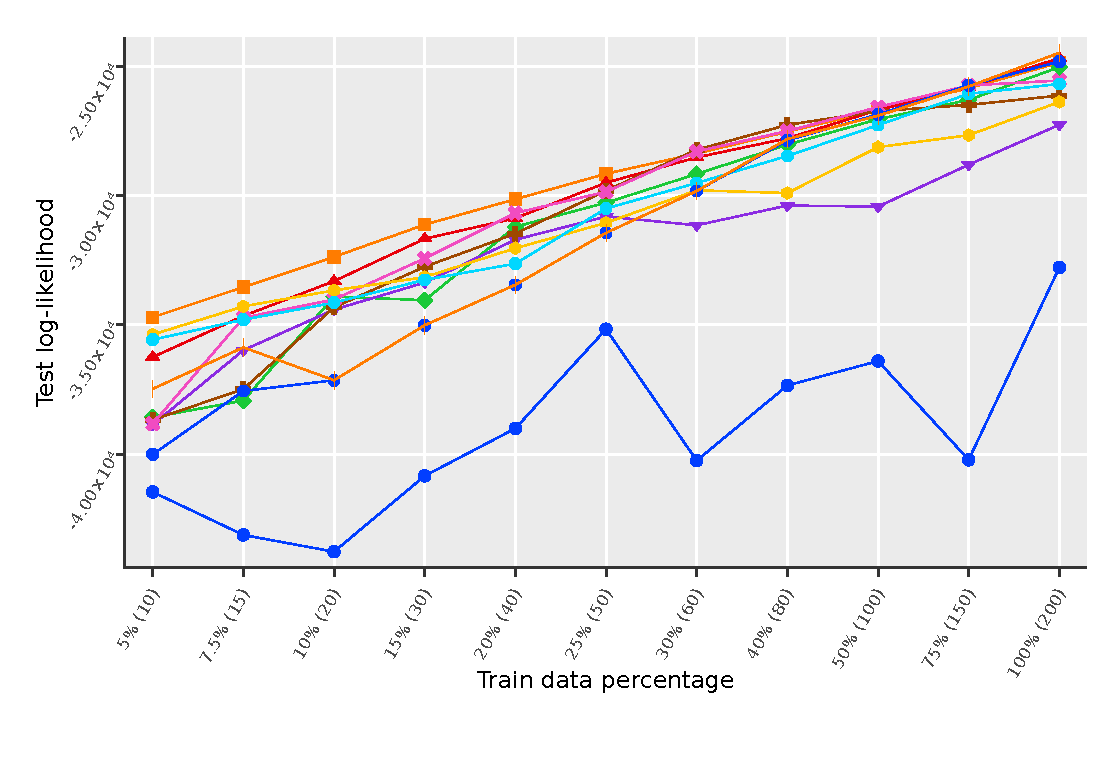
\includegraphics[width=\textwidth]{supplementary/all_ll_led_pixels_ensembles.pdf}
    \caption{}
  \end{subfigure}\\ 
  \begin{subfigure}[b]{0.495\textwidth}
    \centering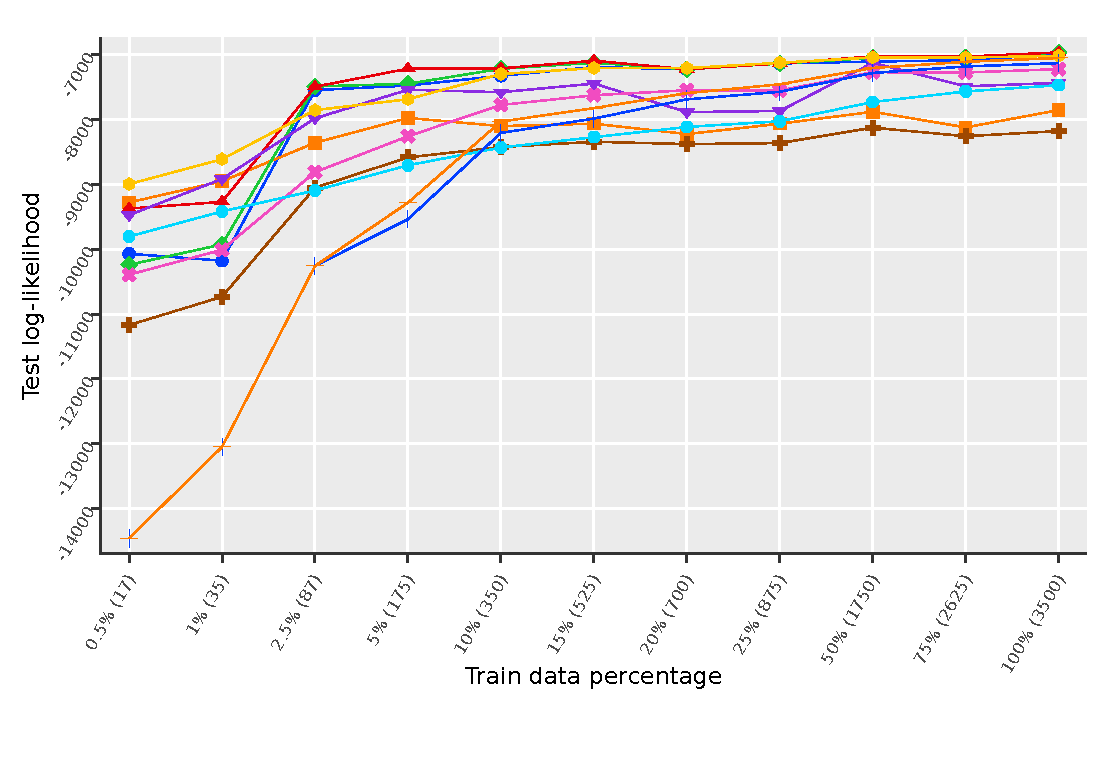
\includegraphics[width=\textwidth]{supplementary/all_ll_sushi_choose_ensembles.pdf}
    \caption{}
  \end{subfigure}
  \begin{subfigure}[b]{0.495\textwidth}
    \centering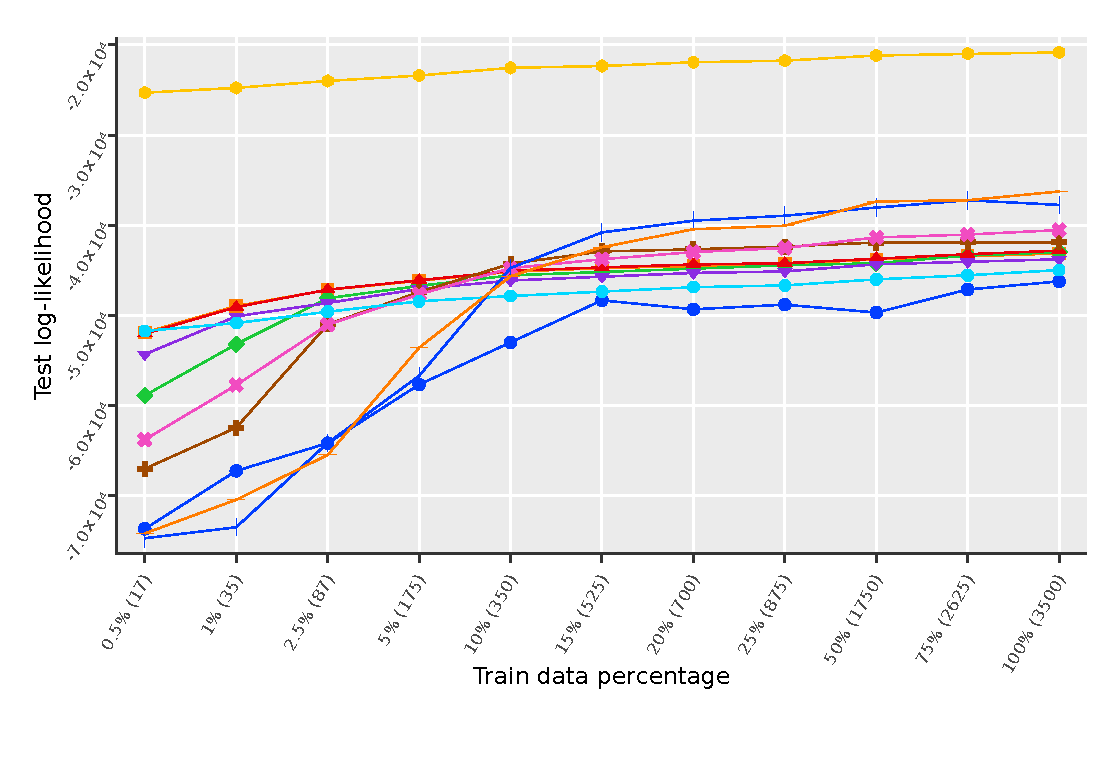
\includegraphics[width=\textwidth]{supplementary/all_ll_sushi_ranking_ensembles.pdf}
    \caption{}
  \end{subfigure}\\
  \begin{subfigure}[t]{0.495\textwidth}
    \centering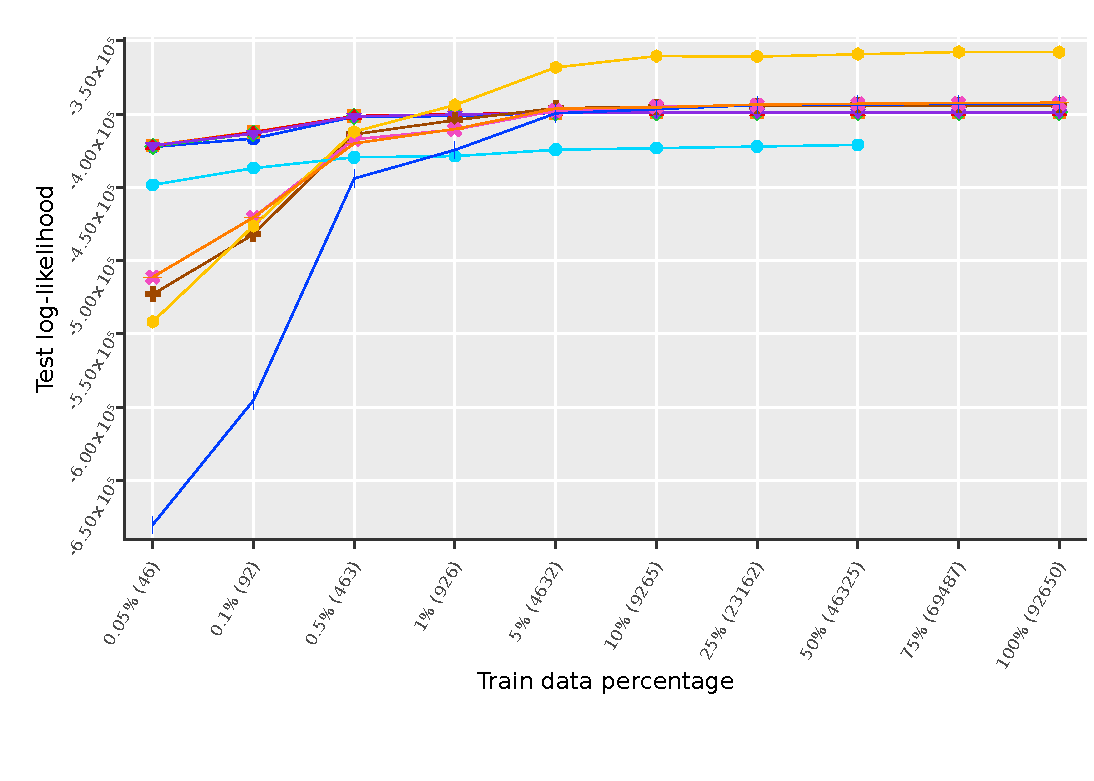
\includegraphics[width=\textwidth]{supplementary/all_ll_dota_ensembles.pdf}
    \caption{}
  \end{subfigure}
  \begin{subfigure}[t]{0.495\textwidth}
    \centering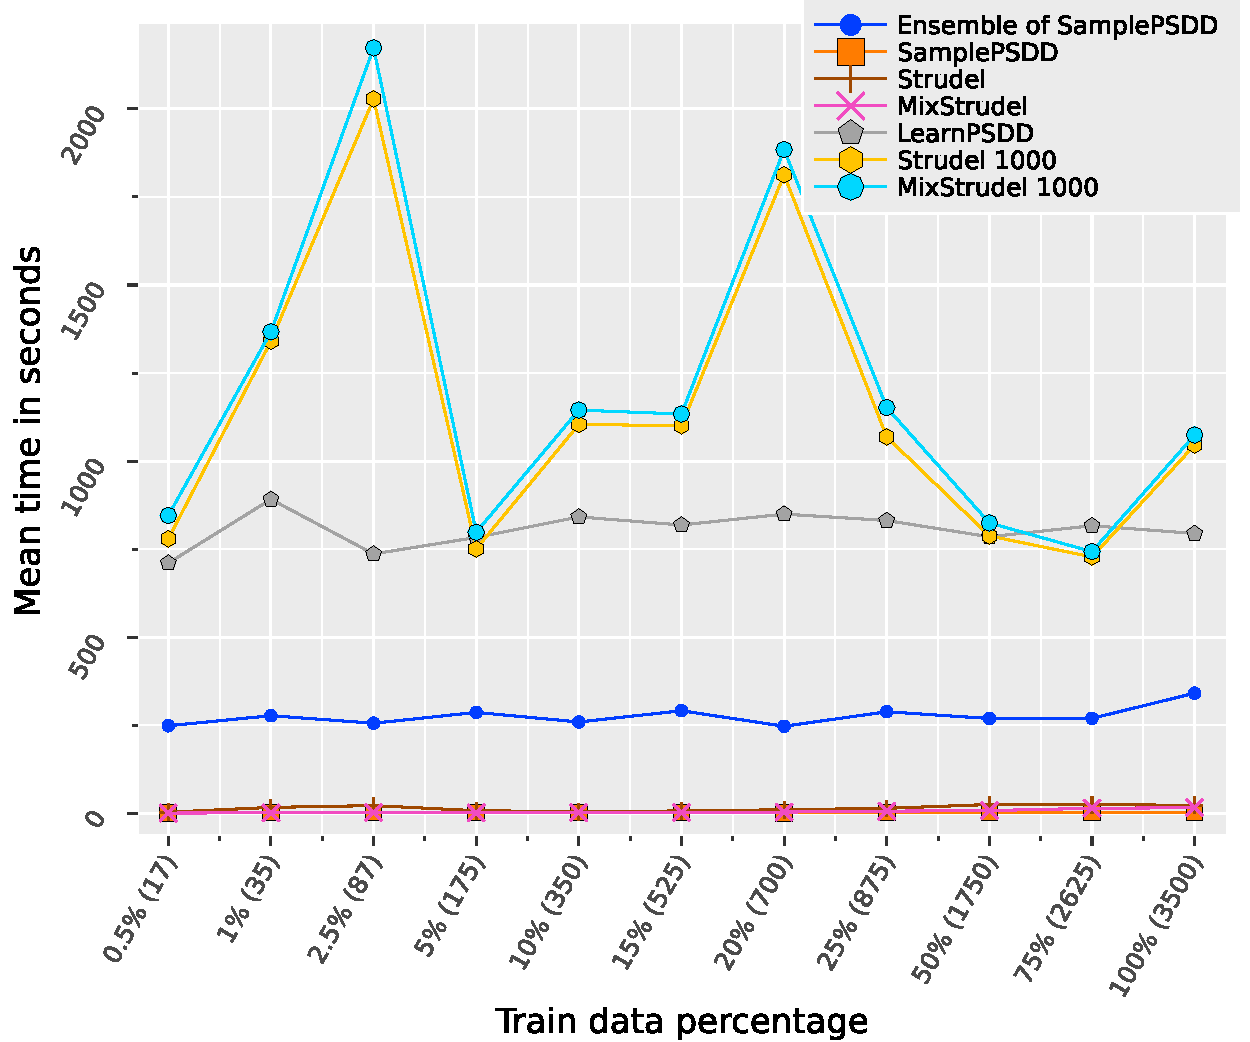
\includegraphics[width=0.9\columnwidth]{supplementary/all_sushi_time.pdf}
    \caption{}
  \end{subfigure}
  \caption{\uncaption{(a)} Log-likelihoods for the unpixelized \texttt{led}, \uncaption{(b)}
    \texttt{led-pixels}, \uncaption{(c)} \texttt{sushi} $10$-choose-$5$, \uncaption{(d)}
    \texttt{sushi} ranking, and \uncaption{(e)} \texttt{dota} datasets. \uncaption{(f)} Mean
    average in seconds of each PSDD learning algorithm.}
  \label{fig:performance}
\end{figure*}

\subsection{Tables with all results}

Tables \ref{tab:all-led} through \ref{tab:all-led-pixels} show all log-likelihood values for all learned
circuits mentioned in the article.

\begin{table*}
  \resizebox{\textwidth}{!} & \textbf{\textsc{LLW}} & \textbf{\textsc{Uniform}} & \textbf{\textsc{EM}} & \textbf{\textsc{Stacking}} & \textbf{\textsc{BMC}} & \textbf{\textsc{Strudel}} & \textbf{\textsc{MixStrudel}} & \textbf{\textsc{CNF}} & \textbf{\textsc{BDD}} & \textbf{\textsc{LearnSPN}} & \textbf{\textsc{Strudel 1000}} & \textbf{\textsc{MixStrudel 1000}} \\
    \hline
    0.02 & -76270.12 & -75787.23 & -84437.88 & -Inf & -76188.67 & -111934.70 & -108848.94 & -63491.43 & -79214.25 & -95691.57 & -97544.40 & -93539.76 \\
    0.05 & -73497.69 & -73346.26 & -73749.15 & -80090.00 & -73134.93 & -98263.88 & -90720.27 & -63601.97 & -79214.25 & -92723.15 & -97544.40 & -93539.76 \\
    0.10 & -71874.12 & -70645.43 & -78218.27 & -72887.26 & -71279.73 & -95780.74 & -86851.08 & -61695.59 & -78972.30 & -87784.83 & -100241.28 & -89465.54 \\
    0.25 & -68850.67 & -65765.90 & -74079.05 & -67914.35 & -66355.85 & -82308.32 & -78892.63 & -64301.48 & -75181.47 & -77728.44 & -101371.88 & -95533.46 \\
    0.50 & -71908.34 & -63836.00 & -67574.64 & -65669.59 & -64123.61 & -79503.19 & -75601.22 & -63489.18 & -75120.22 & -73147.62 & -100880.62 & -100880.62 \\
    0.75 & -68764.98 & -62672.24 & -66423.16 & -63291.72 & -63591.08 & -73509.03 & -71312.21 & -61786.42 & -73306.98 & -71405.55 & -98628.08 & -98628.08 \\
    1.00 & -64046.13 & -62690.14 & -63900.15 & -62744.10 & -62962.83 & -71170.68 & -68344.86 & -63567.95 & -71121.15 & -71979.82 & -97986.81 & -97986.81 \\
    2.50 & -64606.12 & -60058.62 & -64606.01 & -59435.88 & -59623.46 & -61670.14 & -61527.77 & -61817.41 & -68781.20 & -66602.53 & -87585.31 & -83696.90 \\
    5.00 & -59126.68 & -59295.69 & -58950.44 & -58466.21 & -58723.25 & -60542.42 & -59623.12 & -62142.91 & -64901.41 & -63540.15 & -70519.08 & -69183.37 \\
    7.50 & -60206.00 & -59243.14 & -59451.17 & -58280.74 & -58667.93 & -60474.21 & -59302.01 & -63779.07 & -65295.23 & -63461.16 & -65143.38 & -64492.63 \\
    10.00 & -58082.24 & -58990.91 & -58218.28 & -57876.12 & -58603.25 & -59258.70 & -58335.49 & -62272.04 & -63449.87 & -62230.84 & -64059.13 & -62980.20 \\
    25.00 & -58127.23 & -58977.09 & -57827.87 & -57777.27 & -58589.02 & -59116.05 & -58116.16 & -62649.53 & -61490.03 & -60435.37 & -59619.32 & -59663.81 \\
    50.00 & -57683.16 & -58687.88 & -57526.56 & -57512.01 & -58189.97 & -59084.32 & -57654.38 & -63760.85 & -61614.24 & -59703.44 & -58395.85 & -58447.46 \\
    75.00 & -57731.25 & -58900.85 & -57564.91 & -57514.10 & -58416.90 & -59160.69 & -57480.32 & -63656.23 & -61716.55 & -59227.08 & -57947.51 & -58162.58 \\
    100.00 & -57533.82 & -58777.85 & -57444.14 & -57432.12 & -58217.43 & -59140.02 & -57421.31 & -63717.25 & -61823.57 & -58923.36 & -57727.95 & -57921.16 \\
    \hline
  \end{tabular}
  }
  \caption{All results for the \texttt{led} dataset.}
  \label{tab:all-led}
\end{table*}

\begin{table*}
  \resizebox{\textwidth}{!} & \textbf{\textsc{LLW}} & \textbf{\textsc{Uniform}} & \textbf{\textsc{EM}} & \textbf{\textsc{Stacking}} & \textbf{\textsc{BMC}} & \textbf{\textsc{Strudel}} & \textbf{\textsc{MixStrudel}} & \textbf{\textsc{CNF}} & \textbf{\textsc{BDD}} & \textbf{\textsc{LearnSPN}} & \textbf{\textsc{Strudel 1000}} & \textbf{\textsc{MixStrudel 1000}} \\
    \hline
    0.05 & -422502.57 & -421390.69 & -422148.83 & -421743.46 & -421503.71 & -522994.12 & -511269.34 & -- & -541716.99 & -448310.30 & -680217.64 & -511269.34 \\
    0.10 & -416764.85 & -412215.39 & -413252.45 & -412497.30 & -413309.05 & -482048.24 & -470524.47 & -- & -476355.45 & -436929.97 & -595314.50 & -470524.47 \\
    0.50 & -401852.30 & -401428.03 & -401651.98 & -401342.48 & -401639.60 & -413893.71 & -417290.26 & -- & -412120.93 & -429491.77 & -443999.07 & -420096.18 \\
    1.00 & -401399.54 & -400217.55 & -400304.56 & -400241.36 & -400415.36 & -404177.25 & -410592.47 & -- & -393893.11 & -428727.36 & -424539.00 & -410274.56 \\
    5.00 & -399210.71 & -399209.46 & -398999.00 & -398995.65 & -399170.53 & -395999.62 & -397754.60 & -- & -368214.89 & -424401.59 & -399534.98 & -396268.43 \\
    10.00 & -399308.46 & -399114.38 & -399111.18 & -399101.08 & -399139.16 & -394996.70 & -395111.24 & -- & -360499.20 & -423240.08 & -396642.23 & -395462.40 \\
    25.00 & -398759.03 & -398967.54 & -398809.05 & -398789.22 & -398884.48 & -394338.42 & -393943.77 & -- & -360817.30 & -422176.41 & -393840.34 & -393563.40 \\
    50.00 & -398818.59 & -398947.09 & -398781.72 & -398803.82 & -398825.88 & -394185.68 & -393086.71 & -- & -359123.74 & -421069.29 & -393395.77 & -392753.17 \\
    75.00 & -398935.65 & -398983.57 & -398955.77 & -398956.10 & -398958.45 & -394144.51 & -392858.52 & -- & -357708.97 & 0.00 & -393130.99 & -392476.99 \\
    100.00 & -398814.38 & -398946.54 & -398847.74 & -398851.61 & -398903.84 & -394104.98 & -392767.17 & -- & -357820.05 & 0.00 & -393080.77 & -392305.31 \\
    \hline
  \end{tabular}
  }
  \caption{All results for the \texttt{dota} dataset.}
  \label{tab:all-dota}
\end{table*}

\begin{table*}
  \resizebox{\textwidth}{!} & \textbf{\textsc{LLW}} & \textbf{\textsc{Uniform}} & \textbf{\textsc{EM}} & \textbf{\textsc{Stacking}} & \textbf{\textsc{BMC}} & \textbf{\textsc{Strudel}} & \textbf{\textsc{MixStrudel}} & \textbf{\textsc{CNF}} & \textbf{\textsc{BDD}} & \textbf{\textsc{LearnSPN}} & \textbf{\textsc{Strudel 1000}} & \textbf{\textsc{MixStrudel 1000}} \\
    \hline
    0.50 & -10071.51 & -9281.12 & -10241.60 & -9375.70 & -9476.25 & -67065.20 & -63836.65 & -- & -25300.02 & -51765.32 & -14452.67 & -14452.67 \\
    1.00 & -10178.28 & -8954.16 & -9927.91 & -9271.89 & -8919.37 & -62498.23 & -57767.33 & -- & -24760.09 & -50882.04 & -13046.79 & -13046.79 \\
    2.50 & -7551.81 & -8362.66 & -7494.87 & -7498.91 & -7985.90 & -51036.17 & -51070.28 & -- & -23990.52 & -49625.57 & -10259.14 & -10259.14 \\
    5.00 & -7480.58 & -7979.85 & -7454.45 & -7221.24 & -7545.54 & -47444.71 & -47699.34 & -- & -23393.66 & -48465.94 & -9538.90 & -9285.30 \\
    10.00 & -7330.72 & -8105.71 & -7222.63 & -7216.68 & -7583.54 & -44289.65 & -44785.08 & -- & -22534.80 & -47881.50 & -8210.50 & -8035.49 \\
    15.00 & -7196.89 & -8067.99 & -7129.28 & -7099.35 & -7450.98 & -42929.19 & -43793.82 & -- & -22336.59 & -47350.66 & -7989.75 & -7828.43 \\
    20.00 & -7230.35 & -8228.08 & -7230.35 & -7230.13 & -7889.98 & -42692.17 & -42998.28 & -- & -21918.48 & -46898.91 & -7693.88 & -7598.46 \\
    25.00 & -7140.91 & -8068.33 & -7140.90 & -7140.75 & -7872.47 & -42384.75 & -42544.64 & -- & -21738.22 & -46700.17 & -7577.25 & -7461.51 \\
    50.00 & -7111.22 & -7884.88 & -7054.73 & -7031.96 & -7131.19 & -41938.09 & -41373.59 & -- & -21169.19 & -46031.00 & -7286.91 & -7210.35 \\
    75.00 & -7091.82 & -8125.42 & -7043.95 & -7036.04 & -7493.26 & -41931.85 & -41055.14 & -- & -20951.09 & -45576.38 & -7187.18 & -7115.33 \\
    100.00 & -6995.82 & -7859.13 & -6972.82 & -6970.53 & -7439.17 & -41931.72 & -40550.63 & -- & -20824.09 & -44999.66 & -7135.58 & -7055.88 \\
    \hline
  \end{tabular}
  }
  \caption{All results for the \texttt{sushi-ranking} dataset.}
  \label{tab:all-sushi-rank}
\end{table*}

\begin{table*}
  \resizebox{\textwidth}{!} & \textbf{\textsc{LLW}} & \textbf{\textsc{Uniform}} & \textbf{\textsc{EM}} & \textbf{\textsc{Stacking}} & \textbf{\textsc{BMC}} & \textbf{\textsc{Strudel}} & \textbf{\textsc{MixStrudel}} & \textbf{\textsc{CNF}} & \textbf{\textsc{BDD}} & \textbf{\textsc{LearnSPN}} & \textbf{\textsc{Strudel 1000}} & \textbf{\textsc{MixStrudel 1000}} \\
    \hline
    0.50 & -73738.04 & -51933.84 & -58925.72 & -52070.48 & -54347.08 & -11170.18 & -10393.62 & -- & -8998.46 & -9806.06 & -74782.40 & -74245.00 \\
    1.00 & -67295.90 & -48998.01 & -53225.82 & -49112.97 & -50140.36 & -10733.47 & -10010.65 & -- & -8615.35 & -9419.33 & -73557.43 & -70504.16 \\
    2.50 & -64222.40 & -47191.60 & -48124.73 & -47171.38 & -48649.17 & -9054.54 & -8814.77 & -- & -7859.15 & -9097.40 & -64196.67 & -65531.31 \\
    5.00 & -57715.96 & -46215.44 & -46757.26 & -46121.74 & -47099.80 & -8587.40 & -8262.15 & -- & -7692.06 & -8709.09 & -56744.91 & -53619.79 \\
    10.00 & -53029.28 & -45182.87 & -45582.79 & -45096.27 & -46157.73 & -8428.53 & -7779.55 & -- & -7303.22 & -8435.54 & -44767.54 & -45684.07 \\
    15.00 & -48359.59 & -44776.85 & -45173.90 & -44696.40 & -45732.28 & -8346.72 & -7630.41 & -- & -7212.20 & -8272.97 & -40815.68 & -42453.92 \\
    20.00 & -49352.41 & -44503.85 & -44841.65 & -44375.66 & -45316.36 & -8382.45 & -7553.45 & -- & -7213.00 & -8118.19 & -39514.08 & -40466.87 \\
    25.00 & -48837.90 & -44320.47 & -44473.52 & -44232.87 & -45147.34 & -8366.84 & -7558.48 & -- & -7126.86 & -8031.02 & -38959.38 & -40067.63 \\
    50.00 & -49715.52 & -43810.03 & -44236.83 & -43679.79 & -44361.31 & -8129.12 & -7274.86 & -- & -7047.23 & -7733.97 & -38055.99 & -37387.91 \\
    75.00 & -47155.99 & -43439.89 & -43385.69 & -43236.88 & -44080.44 & -8261.48 & -7280.35 & -- & -7050.77 & -7571.72 & -37245.72 & -37239.73 \\
    100.00 & -46253.45 & -43146.33 & -43017.12 & -42836.74 & -43796.68 & -8181.48 & -7227.68 & -- & -7022.86 & -7475.26 & -37761.35 & -36269.11 \\
    \hline
  \end{tabular}
  }
  \caption{All results for the \texttt{sushi-top5} dataset.}
  \label{tab:all-sushi-top}
\end{table*}

\begin{table*}
  \resizebox{\textwidth}{!} & \textbf{\textsc{LLW}} & \textbf{\textsc{Uniform}} & \textbf{\textsc{EM}} & \textbf{\textsc{Stacking}} & \textbf{\textsc{BMC}} & \textbf{\textsc{Strudel}} & \textbf{\textsc{MixStrudel}} & \textbf{\textsc{CNF}} & \textbf{\textsc{BDD}} & \textbf{\textsc{LearnSPN}} & \textbf{\textsc{Strudel 1000}} & \textbf{\textsc{MixStrudel 1000}} \\
    \hline
    5.00 & -41467.80 & -34709.51 & -38580.12 & -36250.22 & -38865.10 & -38681.10 & -38833.61 & -- & -35379.58 & -35577.04 & -40016.81 & -37480.79 \\
    7.50 & -43131.74 & -33541.11 & -37933.14 & -34661.19 & -35984.88 & -37486.80 & -34728.47 & -- & -34287.35 & -34802.33 & -37560.84 & -35873.42 \\
    10.00 & -43778.51 & -32372.82 & -33907.77 & -33312.05 & -34414.20 & -34325.42 & -34019.61 & -- & -33669.67 & -34144.75 & -37146.60 & -37146.60 \\
    15.00 & -40846.42 & -31125.19 & -34049.79 & -31674.03 & -33368.23 & -32755.51 & -32434.84 & -- & -33155.99 & -33261.28 & -35019.44 & -35019.44 \\
    20.00 & -39009.42 & -30139.82 & -31209.07 & -30876.98 & -31708.73 & -31474.09 & -30675.72 & -- & -32038.90 & -32636.76 & -33453.36 & -33453.36 \\
    25.00 & -35170.26 & -29158.72 & -30278.57 & -29505.30 & -30811.56 & -29808.79 & -29856.29 & -- & -31056.47 & -30501.52 & -31443.56 & -31443.56 \\
    30.00 & -40254.35 & -28374.13 & -29166.40 & -28524.61 & -31150.31 & -28229.82 & -28293.39 & -- & -29796.42 & -29515.66 & -29824.86 & -29824.86 \\
    40.00 & -37346.83 & -27532.89 & -28033.83 & -27784.87 & -30386.84 & -27267.30 & -27504.01 & -- & -29904.46 & -28468.36 & -27865.87 & -27815.05 \\
    50.00 & -36404.20 & -26711.99 & -27047.65 & -26693.77 & -30428.74 & -26734.57 & -26579.84 & -- & -28127.06 & -27274.67 & -26863.06 & -26913.21 \\
    75.00 & -40223.88 & -25846.50 & -26300.40 & -25801.80 & -28806.88 & -26494.04 & -25744.18 & -- & -27665.63 & -26064.91 & -25733.69 & -25780.46 \\
    100.00 & -32780.47 & -24858.39 & -25031.07 & -24687.48 & -27260.98 & -26133.39 & -25549.14 & -- & -26379.98 & -25684.45 & -24818.43 & -24478.19 \\
    \hline
  \end{tabular}
  }
  \caption{All results for the \texttt{led-pixels} dataset.}
  \label{tab:all-led-pixels}
\end{table*}



\newpage

\subsection{Logic constraints}

We next show all the logic constraints used for each dataset.

\subsubsection{LED}

\begin{figure}
  \resizebox{\columnwidth}{!}{
  \begin{tikzpicture}
    \node at (0, 0) {\sevensegnum{4}};
    \node at (0, 1) {1};
    \node at (0.75, 0.3) {2};
    \node at (0.75, -0.3) {3};
    \node at (0, -1) {4};
    \node at (-0.75, -0.3) {5};
    \node at (-0.75, 0.3) {6};
    \node at (0, 0.25) {7};
    \node at (5.0, 0.25) {$d_4=\neg X_1\wedge X_2\wedge X_3\wedge\neg X_4\wedge\neg X_5\wedge X_6\wedge X_7$};
    \node at (2.525, -0.5) {$\phi=\bigvee_{i=0}^9 d_i$};
  \end{tikzpicture}
  }
  \caption{LED segment numbering (left), and the corresponding formula for that digit (right).}
\end{figure}

Let $Y_1,Y_2,\ldots,Y_7$ be the observable segments of a 7-segment LED display, with each $Y_i$
representing whether the $i$-th segment (read from the top segment clockwise with the middle
segment last) is observably on (true/1) or off (false/0). We assign a latent variable for each
segment $i$ and call it $X_i$. The latent variable indicates the true intent of the segment (i.e.
whether it was supposed to be on or off regardless of technical problems). For each digit $d_i$, we
add a positive literal if it is supposedly on, and a negative literal if it is supposedly off.
Observable variables are free variables with no constraints. The final formula is given by a
disjunction over all digits, as shown below.

\begin{align*}
\phi=
&\phantom{\neg}X_1 \wedge \phantom{\neg}X_2 \wedge \phantom{\neg}X_3 \wedge \phantom{\neg}X_4 \wedge \phantom{\neg}X_5 \wedge \phantom{\neg}X_6 \wedge \neg X_7 \vee\\
&\neg X_1 \wedge \phantom{\neg}X_2 \wedge \phantom{\neg}X_3 \wedge \neg X_4 \wedge \neg X_5 \wedge \neg X_6 \wedge \neg X_7 \vee\\
&\phantom{\neg}X_1 \wedge \phantom{\neg}X_2 \wedge \neg X_3 \wedge \phantom{\neg}X_4 \wedge \phantom{\neg}X_5 \wedge \neg X_6 \wedge \phantom{\neg}X_7 \vee\\
&\phantom{\neg}X_1 \wedge \phantom{\neg}X_2 \wedge \phantom{\neg}X_3 \wedge \phantom{\neg}X_4 \wedge \neg X_5 \wedge \neg X_6 \wedge \phantom{\neg}X_7 \vee\\
&\neg X_1 \wedge \phantom{\neg}X_2 \wedge \phantom{\neg}X_3 \wedge \neg X_4 \wedge \neg X_5 \wedge \phantom{\neg}X_6 \wedge \phantom{\neg}X_7 \vee\\
&\phantom{\neg}X_1 \wedge \neg X_2 \wedge \phantom{\neg}X_3 \wedge \phantom{\neg}X_4 \wedge \neg X_5 \wedge \phantom{\neg}X_6 \wedge \phantom{\neg}X_7 \vee\\
&\phantom{\neg}X_1 \wedge \neg X_2 \wedge \phantom{\neg}X_3 \wedge \phantom{\neg}X_4 \wedge \phantom{\neg}X_5 \wedge \phantom{\neg}X_6 \wedge \phantom{\neg}X_7 \vee\\
&\phantom{\neg}X_1 \wedge \phantom{\neg}X_2 \wedge \phantom{\neg}X_3 \wedge \neg X_4 \wedge \neg X_5 \wedge \neg X_6 \wedge \neg X_7 \vee\\
&\phantom{\neg}X_1 \wedge \phantom{\neg}X_2 \wedge \phantom{\neg}X_3 \wedge \phantom{\neg}X_4 \wedge \phantom{\neg}X_5 \wedge \phantom{\neg}X_6 \wedge \phantom{\neg}X_7 \vee\\
&\phantom{\neg}X_1 \wedge \phantom{\neg}X_2 \wedge \phantom{\neg}X_3 \wedge \phantom{\neg}X_4 \wedge \neg X_5 \wedge \phantom{\neg}X_6 \wedge \phantom{\neg}X_7
\end{align*}

\subsubsection{LED Pixels}

The LED with pixels dataset follows the same idea as LED, but with added pixels as latent variables
instead of observable segments. We manually observed critical key pixels for each segment (i.e.
pixels which are often set to true/1 if the segment is on. We count pixels row-wise from top left
to bottom right. The following are the critical key pixels for each segment:

\begin{align*}
  S_1&=\{24, 25, 26, 27, 15, 16, 28, 35, 36\}\\
  S_2&=\{27, 28, 37, 38, 47, 48, 57, 58, 49, 59, 69\}\\
  S_3&=\{77, 78, 87, 88, 109, 98, 99, 108, 118\}\\
  S_4&=\{124, 125, 126, 127, 128, 135, 136, 114, 115, 116\}\\
  S_5&=\{93, 94, 103, 104, 113, 114, 124, 82, 92, 83\}\\
  S_6&=\{33, 34, 43, 53, 52, 63, 73\}\\
  S_7&=\{64, 65, 66, 67, 75, 76, 85, 86, 95, 96, 94\}
\end{align*}

Each $S_i$ corresponds to the critical key pixels of segment $i$. The formula for the key pixels
is then set to
\begin{equation*}
  \alpha=\bigvee_{i=1}^7\left(\bigwedge_{p\in S_i}p\right)\wedge X_i.
\end{equation*}

We also add a constraint for pixels which are never on for a given digit. Let $f(i)$ a function
that maps a digit $i$ to the set of all pixels which are always off when $d_i$ is true. We set
\begin{equation*}
  \beta=\bigvee_{i=0}^9 d_i\wedge\left(\bigwedge_{p\in f(i)}\neg p\right).
\end{equation*}

The final constraint is then $\phi=\alpha\wedge\beta$.

\subsubsection{Sushi}

For the sushi ranking dataset, we used the same constraints as \citep{choi15}. For the sushi
10-choose-5, we used the same constraints as \citep{shen17}.

\subsubsection{Dota 2}

To model the constraints, we used a cardinality constraint of $\text{Exactly}(5, 113)$ for the
first and equivalently for the second team. To do this, each character $i$ had a pair of variables
$(X_i,Y_i)$, where $X_i$ attributed the character for the first team, and $Y_i$ to the second. A
cardinality constraint $\sum_{X_i}x_i=5$ was set to the first team, and $\sum_{Y_i}y_i=5$ to the
second.

